\documentclass[10pt,aspectratio=169]{beamer}

\usepackage[T1]{fontenc}
\usepackage{lmodern}

\usepackage{amsmath,amssymb}
\usepackage{bm}
\usepackage{booktabs,tabularx}
\usepackage{graphicx}
\usepackage{hyperref}
\usepackage{xcolor}
\usepackage{tikz}
\usepackage{xspace}

\DeclareMathOperator{\sign}{sign}

\newcommand{\mgut}{\ensuremath{M_{\text{GUT}}}\xspace}
\newcommand{\msusy}{\ensuremath{m_{\text{SUSY}}}\xspace}
\newcommand{\mz}{\ensuremath{M_Z}\xspace}
\newcommand{\mh}{\ensuremath{m_h}\xspace}
\newcommand{\mzero}{\ensuremath{m_0}\xspace}
\newcommand{\mhalf}{\ensuremath{m_{1/2}}\xspace}
\newcommand{\azero}{\ensuremath{A_0}\xspace}
\newcommand{\sgnmu}{\ensuremath{\sign \mu}\xspace}
\newcommand{\gev}{\ensuremath{\,\text{GeV}}\xspace}
\newcommand{\tev}{\ensuremath{\,\text{TeV}}\xspace}
\newcommand{\jac}{\ensuremath{\mathcal{J}}\xspace}

\graphicspath{{./figures/}}

\title{Bayesian analysis and naturalness of (Next-to-)Minimal SUSY Models}

\author{D.~Harries\\
  {\scriptsize
    (IPNP, Charles University in Prague)}\\
  \vspace{25pt}
  { \scriptsize
    Based on: \href{https://doi.org/10.1007/JHEP10(2017)160}{%
      P.~Athron, C.~Bal\'{a}zs, B.~Farmer, A.~Fowlie, D.~Harries,
      and D.~Kim, JHEP \textbf{10}, 160 (2017)}
    [\href{http://arxiv.org/abs/1709.07895}{arXiv:1709.07895}]
  }
}

\titlegraphic{
  \begin{center}
    \hspace*{\fill}
    \includegraphics[scale=0.3]{uk_logo}
    \hspace*{\fill}
  \end{center}
}

\date[Phenomenology 2018, University of Pittsburgh]{May 7, 2018}

\usetheme{CambridgeUS}

\setbeamertemplate{headline}[default]{}
\setbeamertemplate{footline}[page number]{}
\setbeamertemplate{navigation symbols}{}

\begin{document}

\begin{frame}[plain]
  \titlepage
  \usebeamerfont{institute} Contact: \href{mailto:harries@ipnp.mff.cuni.cz}{%
    \texttt{harries@ipnp.mff.cuni.cz}}
\end{frame}

\section{Naturalness Measures}

\begin{frame}
  \frametitle{Naturalness Problems}
  \begin{columns}[t]
    \begin{column}{0.5\textwidth}
      \begin{itemize} \itemsep1em
        \item Common motivation for SUSY is the hierarchy problem,
      \end{itemize}
      \begin{center}
        \includegraphics[width=0.8\textwidth]{fermionloop}
      \end{center}
      \begin{itemize} \itemsep1em
      \item Example of a \alert{``naturalness problem''}
        \begin{itemize}
        \item See also: strong CP problem, cosmological constant
          problem, flatness problem, $\ldots$
        \end{itemize}
      \end{itemize}
    \end{column}
    \begin{column}{0.5\textwidth}
      \begin{itemize} \itemsep1.5em
      \item Possible characterisation: {\color{blue} propensity of model to
        reproduce data}
      \item Related to \alert{fine-tuning}, e.g., if observations require
        a priori unjustified tuning of parameters $\Rightarrow$ model
        unnatural
      \item Prefer models in which fine-tuning not required/reduced?
      \item E.g., ``little hierarchy problem'' in MSSM
        (at tree-level)
        \begin{equation*}
          m_{h_1}^2 \leq m_Z^2 \cos^2 2\beta \, { \color{red} \lesssim
            (91 \text{ GeV})^2}
        \end{equation*}
        {\color{blue} $\Rightarrow$ non-minimal SUSY models?}
      \end{itemize}
    \end{column}
  \end{columns}
\end{frame}

\begin{frame}
  \frametitle{Quantifying Fine-tuning}
  \begin{block}{Typical Motivation}
    <model name> raises the Higgs mass at tree-level, and
    therefore is more natural than the MSSM, e.g., in the NMSSM
    \begin{equation*}
      m_{h_1}^2 \lesssim m_Z^2 \cos^2 2\beta + \frac{\lambda^2 v^2}{2}
      \sin^2 2\beta
    \end{equation*}
  \end{block}
  \begin{itemize} \itemsep1em
  \item Justify/check claim that model is more natural than another
    $\Rightarrow$ quantify naturalness, i.e., fine-tuning
  \item Traditionally, construct {\color{blue} fine-tuning measure}, i.e.,
    calculable function of model parameters that is identified with tuning
  \item Focus on different features of a model's behaviour $\Rightarrow$
    different fine-tuning measure
    \begin{itemize}
    \item Model fine-tuned according to one measure $\Rightarrow$ also
      fine-tuned under a different measure?
    \end{itemize}
  \item \alert{I.e., depends on your definition of fine-tuning $\ldots$}
  \end{itemize}
\end{frame}

\begin{frame}
  \frametitle{Traditional Tuning Measures}
  \begin{center}
    What constitutes "fine-tuning"? \\
    Opinions differ.
  \end{center}
  \begin{itemize} \itemsep0.8em
    \item Large cancellations [1]?
      \begin{equation*}
        \Delta_{EW} = \max_i \frac{2|C_i|}{m_Z^2}, \quad C_1 = -\mu^2, \,
        C_2 = \frac{m_{H_d}^2}{\tan^2\beta - 1}, \ldots
      \end{equation*}
    \item Extreme sensitivities [2]?
      \begin{equation*}
        \Delta_{BG} = \max_i \left | \frac{\partial \ln m_Z^2}
        {\partial \ln p_i} \right | , \quad p_i \in \{\text{fundamental
        parameters}\}
      \end{equation*}
    \item High or low energy contributions ($\Delta_{EW}$ or $\Delta_{HS}$)?
      Definition of parameters $p_i$? Just $m_Z$?
    \item Model fine-tuned $\Leftrightarrow \Delta_{EW/HS/BG/\ldots} > ?$
    \item Compare tuning between models?
  \end{itemize}
  \begin{center}
  \alert{What does $\Delta_{EW/HS/BC/\ldots} > x$ mean for our degree of belief
    in model?}
  \end{center}
      { \tiny
        [1] H.~Baer, V.~Barger, P.~Huang, A.~Mustafayev, and X.~Tata,
        \href{https://doi.org/10.1103/PhysRevLett.109.161802}{%
          Phys.~Rev.~Lett.~\textbf{109} (2012) 161802}
             [\href{http://arxiv.org/abs/1207.3343}{arXiv:1207.3343}] \\[-5pt]
        [2] J.~R.~Ellis, K.~Enqvist, D.~V.~Nanopoulos, and F.~Zwirner,
        \href{https://doi.org/10.1142/S0217732386000105}{%
          Mod.~Phys.Lett.~\textbf{A1} (1986) 57};
          R.~Barbieri and G.~F.~Giudice,
          \href{https://doi.org/10.1016/0550-3213(88)90171-X}{%
            Nucl.~Phys.~\textbf{B306} (1988) 63}
      }
\end{frame}

\begin{frame}
  \frametitle{Traditional Tuning Measures}
  \begin{columns}[t]
    \begin{column}{0.5\textwidth}
      \begin{figure}
        \centering
        \includegraphics[width=\textwidth]{msugra_measures_comparison}
      \end{figure}
    \end{column}
    \begin{column}{0.5\textwidth}
      \begin{figure}
        \centering
        \includegraphics[width=\textwidth]{nuhm2_measures_comparison}
      \end{figure}
    \end{column}
  \end{columns}
  \begin{center}
    \tiny
        [\href{http://arxiv.org/abs/1309.2984}{arXiv:1309.2984}]
  \end{center}
\end{frame}

\section{Bayesian Naturalness}

\begin{frame}
  \frametitle{A Bayesian Approach}
  \begin{itemize} \itemsep1.1em
  \item Results based on traditional measures depend heavily on
    choice of measure
  \item Generally, when we talk about ``naturalness'' we are really
    talking about plausibility
    \begin{itemize} \itemsep0.8em
    \item Unnatural model $\Leftrightarrow$ implausible model
    \item \alert{Traditional measures do not have an unambiguous interpretation
      in this sense}
    \end{itemize}
  \item $\Rightarrow$ better questions to ask are,
    \vspace{7pt}
    \begin{center}
      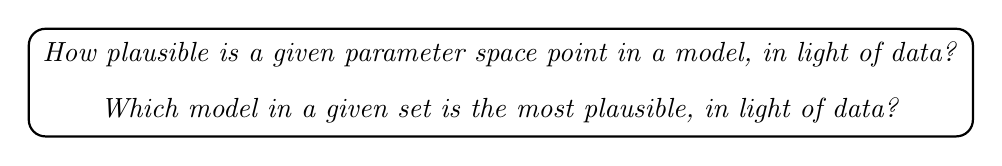
\begin{tikzpicture}
        \node[rectangle, draw, fill = white, rounded corners = 6pt,
          thick, inner sep = 0.5em, align = center]{
          \textit{How plausible is a given parameter space point in a model,
            in light of data?}\\[0.8em]
          \textit{Which model in a given set is the most plausible, in light
            of data?}
        };
      \end{tikzpicture}
    \end{center}
  \item {\color{blue} Rigorous logical framework exists for answering these
    questions: Bayesian statistics}
  \end{itemize}
\end{frame}

\begin{frame}
  \frametitle{Naturalness Priors}
  \begin{itemize} \itemsep1em
  \item Bayesian framework {\color{blue} automatically captures
    intuition about ``naturalness''}
  \item Bayes' theorem applied to model $M$, parameters $\bm{x}$,
    "observables" $\bm{O}$:
    \begin{gather*}
      p(\bm{x}|\text{data},M) = \frac{p(\text{data}|\bm{x},M) p(\bm{x}|M)}
      {p(\text{data}|M)} , \quad
      p(M|\text{data}) = \frac{p(\text{data}|M) p(M)}{p(\text{data})} \\
      {\color{orange} p(\text{data}|M)}
      = \int d^n x_i\; p(\text{data}|
      \bm{x},M) p(\bm{x}|M), \quad
         {\color{green} p_{\text{eff.}}(x_j,\ldots)} = \int dO_i \;
         p(\bm{O}, \bm{x}^\prime | M, O_i^{\text{exp.}})
    \end{gather*}
  \item Reparameterise in favour of $\bm{O}$ and remaining parameters
    $\bm{x}^\prime$, e.g.,
    \begin{equation*}
      p(\bm{x}|M) = \mathcal{J} p(\bm{O},\bm{x}^\prime|M)
    \end{equation*}
    $\Rightarrow$ {\color{orange} evidence} and {\color{green}
      effective naturalness priors} {\color{blue} suppressed by Jacobian}
    $\Delta_J \sim \mathcal{J}$ [3],
    \begin{equation*}
      \Delta_J = \left | \det \frac{\partial \ln O_i}{\partial \ln x_j}
      \right |
    \end{equation*}
  \end{itemize}
      {
        \tiny
        [3] D.~Kim, P.~Athron, C.~Bal\'{a}zs, B.~Farmer, and E.~Hutchison,
        \href{https://doi.org/10.1103/PhysRevD.90.055008}{%
          Phys.~Rev.~D \textbf{90} (2014) 055008}
        [\href{http://arxiv.org/abs/1312.4150}{arXiv:1312.4150}]
      }
\end{frame}

\begin{frame}
  \frametitle{Example: the SM Hierarchy Problem}
  \begin{columns}[t]
    \begin{column}{0.5\textwidth}
      \vspace{-15pt}
      \begin{center}
        Toy model $\Rightarrow$ $M_Z^2 = -\frac{\bar{g}^2}{8 \lambda} (\mu^2
        + \Lambda_{NP}^2)$
      \end{center}
      \vspace{-10pt}
      \begin{figure}
        \includegraphics[width=0.9\textwidth]{SM_Lambda}
      \end{figure}
      \vspace{-20pt}
      \begin{center}
        \tiny
        [\href{http://arxiv.org/abs/1709.07895}{arXiv:1709.07895}]
      \end{center}
    \end{column}
    \begin{column}{0.5\textwidth}
      \begin{itemize} \itemsep1em
      \item Traditional BG measure applied to, e.g., cut-off $\Lambda_{NP}^2$,
        \begin{equation*}
          \Delta_{\Lambda_{NP}^2} = \frac{\bar{g}^2}{8 \lambda}
          \frac{\Lambda_{NP}^2}{M_Z^2}
        \end{equation*}
        $\Rightarrow$ large tuning for $\Lambda_{NP}^2 \gg M_Z^2$
        \alert{but interpretation unclear}
      \item Compute posterior for $\Lambda_{NP}^2$ using
        \begin{equation*}
          p_{\text{eff.}}(\Lambda^2, \lambda) \propto
          \left | \frac{\partial M_Z}{\partial \mu^2}
          \right |^{-1}_{\mu = \mu_Z} p(\Lambda^2, \mu_Z^2, \lambda | SM)
        \end{equation*}
      $\Rightarrow$ captures traditional intuition about tuning
      \item {\color{blue} But also has a well-defined probabilistic
        interpretation}
      \end{itemize}
    \end{column}
  \end{columns}
\end{frame}

\section{Results}

\begin{frame}
  \frametitle{Models Considered}
  \begin{columns}[t]
    \begin{column}{0.55\textwidth}
      \vspace{-10pt}
      \begin{itemize} \itemsep1em
      \item CMSSM as reference model with parameters
        $\mu_0$, $B_0 \mu_0$, $\sgnmu$, and
        \begin{gather*}
          m_Q^2 = m_{u^c}^2 = \ldots = m_{H_d}^2 = m_{H_u}^2 = \mzero^2 , \\
          M_1 = M_2 = M_3 = \mhalf , \\
          A_u = A_d = A_e = \azero
        \end{gather*}
      \item Naturalness priors from $\{ |\mu_0 |, B_0 \mu_0 \}
        \to \{ M_Z^2, \tan\beta \}$
      \item Semi-constrained $\mathbb{Z}_3$-NMSSM,
        \begin{equation*}
          \widehat{W}_{\text{NMSSM}} = \left . \widehat{W}_{\text{MSSM}}
          \right |_{\mu = 0} + \lambda \hat{S} \hat{H}_d \cdot \hat{H}_u
          + \frac{1}{3} \kappa \hat{S}^3 ,
        \end{equation*}
        new parameters $\lambda_0$, $\kappa_0$, $m_{S_0}^2$,
        $\sign (\lambda \langle S \rangle)$,
        $A_\lambda$, $A_\kappa$
      \item Trade $\{ \lambda_0, \kappa_0, m_{S_0}^2 \}
        \to \{ \lambda, M_Z^2, \tan\beta \}$
      \end{itemize}
    \end{column}
    \begin{column}{0.5\textwidth}
      \begin{table}
        \centering
        \begin{tabularx}{0.8\textwidth}{cX}
          \toprule
          CMSSM\\
          \midrule
          \mzero & Log, $1\gev - 20\tev$\\
          \mhalf & Log, $1\gev - 15\tev$\\
          \azero & \parbox[c]{\textwidth}{Log,
            $100 \gev < |A| \le 20\tev$,\\
            Flat, $|A| \le 100 \gev$}\\
          $|\mu_0|$ & Log, $100\gev-20\tev$\\
          $B_0\mu_0$ & Log, $(100\gev)^2-(20\tev)^2$\\
          \sgnmu & $\pm1$ with equal probability\\
          \midrule
          NMSSM\\
          \midrule
          $\lambda_0$ & Log, $10^{-6}-1$\\
          $\kappa_0$ & Log for $10^{-10}< |\kappa| < 1$\\
          $m_{S_0}$ & Same as $\mzero$\\
          $A_\lambda$ & Same as \azero\\
          $A_\kappa$ & Same as \azero\\
          \bottomrule
        \end{tabularx}
      \end{table}
    \end{column}
  \end{columns}
\end{frame}

\begin{frame}
  \frametitle{Low Fine-tuning and Credible Regions}
  \begin{columns}[t]
    \begin{column}{0.7\textwidth}
      \begin{columns}[t]
        \begin{column}{0.5\textwidth}
          \vspace{-35pt}
          \begin{figure}
            \centering
            \includegraphics[width=0.8\textwidth]{CMSSM_BG_m0m12}
          \end{figure}
          \vspace{-20pt}
          \begin{figure}
            \centering
            \includegraphics[height=0.7\textwidth]{CMSSM_pdf_mz_m0m12}
          \end{figure}
        \end{column}
        \begin{column}{0.5\textwidth}
          \vspace{-35pt}
          \begin{figure}
            \centering
            \includegraphics[width=0.8\textwidth]{CNMSSM_BG_m0m12}
          \end{figure}
          \vspace{-20pt}
          \begin{figure}
            \centering
            \includegraphics[height=0.7\textwidth]{CNMSSM_pdf_mz_m0m12}
          \end{figure}
        \end{column}
      \end{columns}
      \vspace{-12pt}
      \begin{center}
        \tiny [\href{http://arxiv.org/abs/1709.07895}{arXiv:1709.07895}]
      \end{center}
    \end{column}
    \begin{column}{0.3\textwidth}
      \vspace{-25pt}
      \begin{figure}
        \centering
        \includegraphics[height=0.9\textwidth]{CNMSSM_mh}
      \end{figure}
      \vspace{-10pt}
      \begin{itemize} \itemsep1em
      \item {\color{blue} High posterior density $\Leftrightarrow$ low
        fine-tuning (according to $\Delta_{BG}$)}
      \item $m_{h_1} \approx 125$ GeV not required $\Rightarrow$
        weak-scale soft parameters preferred
      \end{itemize}
    \end{column}
  \end{columns}
\end{frame}

\begin{frame}
  \frametitle{Impact of $m_h \approx 125$ GeV}
  \begin{columns}[t]
    \begin{column}{0.7\textwidth}
      \begin{columns}[t]
        \begin{column}{0.5\textwidth}
          \vspace{-35pt}
          \begin{figure}
            \centering
            \includegraphics[width=0.8\textwidth]{CMSSM_BG_mh_m0m12}
          \end{figure}
          \vspace{-20pt}
          \begin{figure}
            \centering
            \includegraphics[height=0.7\textwidth]{CMSSM_pdf_mz_mh_m0m12}
          \end{figure}
        \end{column}
        \begin{column}{0.5\textwidth}
          \vspace{-35pt}
          \begin{figure}
            \centering
            \includegraphics[width=0.8\textwidth]{CNMSSM_BG_mh_m0m12}
          \end{figure}
          \vspace{-20pt}
          \begin{figure}
            \centering
            \includegraphics[height=0.7\textwidth]{CNMSSM_pdf_mz_mh_m0m12}
          \end{figure}
        \end{column}
      \end{columns}
      \vspace{-12pt}
      \begin{center}
        \tiny [\href{http://arxiv.org/abs/1709.07895}{arXiv:1709.07895}]
      \end{center}
    \end{column}
    \begin{column}{0.3\textwidth}
      \begin{itemize} \itemsep1em
      \item \alert{Credible intervals shifted $\sim 2$ orders of magnitude in
        \mzero, \mhalf}
        \begin{itemize} \itemsep0.8em
        \item Expected: LHC  $\Rightarrow$ SUSY implausible below $\sim 1$ TeV
        \end{itemize}
      \item Still find most plausible regions $\Leftrightarrow$ lowest
        tunings {\color{blue} consistent with data}
      \item Both approaches $\Rightarrow$ focus-point region is preferred
      \end{itemize}
    \end{column}
  \end{columns}
\end{frame}

\begin{frame}
  \frametitle{Comparing Fine-tuning Measures}
  \begin{columns}[t]
    \begin{column}{0.3\textwidth}
      \begin{figure}
        \centering
        \includegraphics[width=\textwidth]{CNMSSM_BG_mh_m0m12}
      \end{figure}
    \end{column}
    \begin{column}{0.3\textwidth}
      \begin{figure}
        \centering
        \includegraphics[width=\textwidth]{CNMSSM_EW_mh_m0m12}
      \end{figure}
      \vspace{-15pt}
      \begin{center}
        \tiny [\href{http://arxiv.org/abs/1709.07895}{arXiv:1709.07895}]
      \end{center}
    \end{column}
    \begin{column}{0.3\textwidth}
      \begin{figure}
        \centering
        \includegraphics[width=\textwidth]{CNMSSM_GUT_J_mh_m0m12}
      \end{figure}
    \end{column}
  \end{columns}
  \begin{columns}[t]
    \begin{column}{0.5\textwidth}
      \begin{itemize} \itemsep1em
      \item Can use $\Delta_J$ as a standalone tuning measure
      \item {\color{blue}Qualitative agreement between $\Delta_{BG}$,
        $\Delta_{EW}$, $\Delta_J$}
      \item \alert{But meaningful results $\Rightarrow$ ideally
        should compute full posterior densities or evidences}
      \end{itemize}
    \end{column}
    \begin{column}{0.5\textwidth}
      \begin{itemize} \itemsep1em
      \item Some differences, e.g., $\Delta_J$ shows much stronger
        preference for focus point than $\Delta_{BG}$
      \item Aside: differing definitions of measures $\Rightarrow$ direct
        comparison of values not reasonable
      \end{itemize}
    \end{column}
  \end{columns}
\end{frame}

\begin{frame}
  \frametitle{Posterior Distributions}
  \begin{columns}[t]
    \begin{column}{0.3\textwidth}
      \vspace{-20pt}
      \begin{figure}
        \centering
        \includegraphics[width=\textwidth]{CNMSSM_mz_violin}
      \end{figure}
    \end{column}
    \begin{column}{0.3\textwidth}
      \vspace{-20pt}
      \begin{figure}
        \centering
        \includegraphics[width=\textwidth]{CNMSSM_mzmh_violin}
      \end{figure}
      \vspace{-15pt}
      \begin{center}
        \tiny [\href{http://arxiv.org/abs/1709.07895}{arXiv:1709.07895}]
      \end{center}
    \end{column}
    \begin{column}{0.3\textwidth}
      \vspace{-20pt}
      \begin{figure}
        \centering
        \includegraphics[width=\textwidth]{CMSSM_mzmh_violin}
      \end{figure}
    \end{column}
  \end{columns}
  \begin{columns}[t]
    \begin{column}{0.5\textwidth}
      \begin{itemize} \itemsep0.7em
      \item {\color{blue} Posterior densities reflect traditional
        intuition}
      \item Pre-Higgs densities $\Rightarrow$ low $\msusy \lesssim
        1 \tev$ most plausible (``natural'')
      \item Inclusion of $m_h$ $\Rightarrow$ $\msusy \gtrsim 4 \tev$
        required, TeV scale soft parameters
      \end{itemize}
    \end{column}
    \begin{column}{0.5\textwidth}
      \begin{itemize} \itemsep0.7em
      \item {\color{blue} Bayesian approach $\Rightarrow$
        systematically update degree of belief given new data}
      \item \alert{Ambiguous when using approach based on
        $\Delta_{EW/BG/\ldots}$}
      \end{itemize}
    \end{column}
  \end{columns}
\end{frame}

\section{Summary}

\begin{frame}
  \frametitle{Summary}
  \begin{itemize} \itemsep1em
  \item Model comparison based on traditional tuning measures is
    ill-defined
  \item More relevant to ask which parameter values/models are
    most plausible given observations $\Rightarrow$ utilitise Bayesian
    methods
  \item Bayesian approach automatically incorporates traditional
    intuitions about fine-tuning
  \item {\color{blue} Effective naturalness priors resemble traditional
    measures but have a rigorous probabilistic interpretation}
  \item Qualitative agreement between traditional measures and naturalness
    priors, credible intervals in the CMSSM and semi-constrained NMSSM
  \item In principle, can go further: have all ingredients to
    compare model evidences $\Rightarrow$ {\color{blue} statistically
      meanginful model comparisons}
  \end{itemize}
  \begin{center}
    \large Thank you for listening!
  \end{center}
\end{frame}

\appendix

\begin{frame}
  \begin{center}
    {
      \Large
      Additional Slides
    }
  \end{center}
\end{frame}

\begin{frame}
  \frametitle{Minimum Tuning Values}
  \begin{table}[htbp]
    \centering
    \begin{tabular}{lcccc}
      \toprule
      & \multicolumn{2}{c}{\mz}
      & \multicolumn{2}{c}{\mz and $\mh \approx 125\gev$} \\
      \cmidrule(r){2-3}\cmidrule(r){4-5}
      & CMSSM & NMSSM & CMSSM & NMSSM\\
      \midrule
      $\Delta_J\big|_{\mgut}$ & $3 \times 10^{-9}$
      & $2 \times 10^{-10}$ & $0.004$ & $8 \times 10^{-7}$ \\
      $\Delta_J\big|_{\msusy}$ & $6 \times 10^{-7}$
      & $2 \times 10^{-10}$ & $0.005$ & $8 \times 10^{-7}$ \\
      $\Delta_{EW}$ & $0.3$ & $0.3$ & $48.7$ & $47.4$ \\
      $\Delta_{BG}$ & $0.1$ & $0.2$ & $451.9$ & $133.2$ \\
      \bottomrule
    \end{tabular}
  \end{table}
  \begin{itemize} \itemsep1em
  \item \alert{Note: numbers should be compared keeping in mind differing
    definitions of measures}
  \item $\Delta_J \big|_{\msusy}$ $\Rightarrow$ contributions to Jacobian
    from RG running omitted
  \item All measures increase once $m_h$ included
  \item Note $\Delta_{EW}$ similar for both models, while $\Delta_{BG}$,
    $\Delta_J$ smaller for NMSSM
  \end{itemize}
\end{frame}

\end{document}
